\chapter{\uppercase{Background on Data-Consistent Inversion} \label{chapter:02}}

\section{Notation, Terminology, and Assumptions}
We begin by assuming that a (deterministic) model, denoted by $$\M (u, \param) = 0,$$ is specified to relate observable state variables $u$ to model inputs ({\em parameters}) denoted by the vector $\param\in\RP$.
The components $\param_\iparam$ may include parameters in either the model operator (e.g. a diffusion coefficient) or input data (e.g. the frequency of a sinusoidal source, initial, or boundary information).
We allow $\pspace$ to denote the set of all possible input parameters.
We assume $\pspace\subset\RP$ is equipped a (volume) measure, $\pmeas$ on the Borel $\sa$ $\pborel$, defining the measure space $\Pspace$.
The solution operator of the model $\M$ then defines a map taking $\param\in\pspace$ to a solution denoted $u\lam$ which is assumed to be unique.

However, in real experimental settings we are often unable to observe $u\lam$, instead having access to some finite set of observable scalar quantities.
For example, in experiments involving the diffusion of heat, we can typically only record the temperature at some small number of pre-specified points in space-time where measurement devices can be positioned.

Such observable values of $u\lam$ are mathematically modeled by functionals of the solution, denoted $\qoi_\idata: u\lam \to \RR$.
The collection of such functionals into a vector defines a {\em Quantity of Interest} (QoI) map.
Since the solution to the model depends on $\param$, so do the QoI, which motivates the notation
$$\qlam := \qoi( u\lam ) \in\RD,$$
to make this dependence on model parameters explicit.
Furthermore, this convention captures a realistic limitation of an experimental setting, where we may be able to control $\param$ in order to observe $\qlam$, but lack the ability to observe $u\lam$ directly.
The outputs of the QoI map $\qlam = \data$ are what we refer to as the \emph{data}.
Similarly, the range of the QoI defines the \emph{data space} $\dspace$, i.e.
$$\dspace = \qoi(\pspace) \subset \RD$$

We let $\qspace$ denote the set of possible QoI maps for which it is possible to collect experimental data.
For example, suppose we may record only a single temperature measurement at any of ten locations in space-time.
Then $\qspace$ is defined by ten possible QoI maps.
If we can record any two such measurements, then $\qspace$ is defined by $\binom{10}{2} = 45$ possible maps.
Observe that $\qspace$ could easily be uncountable, for example if we were not limited to the spatial locations (or time) at which we could record temperature measurements.
However, for simplicity, we will only discuss problems where $\qspace$ is finite.
In the event that we need to compare maps, we adopt the notation $\dspace_{\qoi}$ to emphasize that the data space depends on the choice of QoI map $\qoi$; when the context is clear, we drop the subscript.
The only assumption on $\qoi$ that we impose throughout this work is that of piecewise-differentiability.


%%%%%%%%%%%%%%%%%%%%%%%%%%%%%%%%%%%%%%%%%%%%%%%%%%%%%%%%%%%%%%%%%%%%%%
\pagebreak
\section{Set-Based Inversion for Measures}\label{sec:ch02-set}
To properly summarize the Stochastic Inverse Problem (SIP) and desired solution, we define several measure/probability spaces and refer to the schematic given in Figure \ref{fig:scheme}\---borrowed from \cite{BM17}\---in order to illustrate the steps and spaces required in the formulation and solution of the SIPs we consider herein.
For a more extensive review, we refer the reader to \cite{BBE11}, \cite{BES12}, \cite{BET+14}, and \cite{BM17}.

%%%%%%%%%%%%%%%%%%%%%%%%
\begin{figure}[!h]
\begin{equation}
\underbrace{
\underbrace{
\overbrace{
 \Pspace \xmapsto{\  Q \ } \Dspace
  \xmapsto{\ \dataP \ } (\dspace, \dborel, \dataP)
 }^{
 \text{(S1): Stochastic Inverse Problem (SIP)}
 }
 \xmapsto{\ Q^{-1} \ } (\pspace, \cborel, \contourP)
 }_{
 \text{(S2): Solution to SIP Satisfying Eq. \eqref{eq:dataspace_pushforward_measure}}}
 \xmapsto{\ \set{\PP_\ell}_{\ell\in\mathcal{L}} \ } (\pspace, \pborel, \paramP)
 }
 _{
 \text{(S3): Unique Solution to SIP by Eq.~\eqref{eq:disintegration_measure} and Ansatz}
 }
\end{equation}
\caption{The first step (S1) defines (i)~the formulation of the SIP by specification of the model, (ii)~the measure spaces of parameters and (iii)~observable outputs, and (iv)~the probability measure on the latter. The second step (S2) defines a unique solution to the SIP on the space $\pspace$ equipped with the contour $\sa$ $\cborel$ using the definition of the push-forward measure. In (S3), the Disintegration Theorem and and Ansatz are applied to define a unique solution on the space of interest $(\pspace, \pborel)$ equipped with a probability measure $\paramP$.}
\label{fig:scheme}
\end{figure}


The initial measure/probability spaces involved in the formulation of the SIP are summarized in step (S1) of Fig.~\ref{fig:scheme}, starting with measure space $\Pspace$.

The assumption that $\qoi$ is at least piecewise-differentiable implies the measurability of the QoI map, so that the space $\dspace$ induced by $\qoi$ is equipped with the Borel $\sa$ $\dborel$ [TK - cite textbook].
The ``push-forward'' measure $\dmeas$ on ${(\dspace, \dborel)}$ is defined as
\begin{equation}\label{eq:dataspace_pushforward_measure}
\dmeas (A) = \int_A \, d\dmeas := \int_{\qoi^{-1}(A)} \, d\pmeas = \pmeas \left (\qoi^{-1}(A) \right ) \quad \forall \;  A\in\dborel,
\end{equation}
which defines the measure space $\Dspace$\footnote{When referring to properties of the data space that are not unique to the choice of map used to induce $\dspace$, we will drop the subscript notation and assume the dependence is understood, as expressed in Fig.~\ref{fig:scheme}.}.
The push-forward distribution $\partial \dataP / \partial \mu_D$ is referred to as the \emph{predicted} distribution and is given by the Radon-Nikodym derivative with respect to (the Lebesgue) volume measure $\mu_D$ on ${(\dspace, \dborel)}$

The final step in (S1) involves the specification of a probability measure $\dataP$ on ${(\dspace, \dborel)}$ to model the uncertainty in data.
We colloquially refer to the distribution (given by the Radon-Nikodym derivative $\partial \dataP / \partial \pmeas$) as the \emph{observed} distribution, where $\pmeas$ is taken to be the (Lebesgue) volume measure on ${(\pspace, \pborel)}$.
This leads to the following SIP: determine a probability measure $\paramP$ on ${(\pspace, \pborel)}$ such that the push-forward measure of $\paramP$ matches $\dataP$.

In other words, determine a $\paramP$ satisfying
\begin{equation}\label{eq:inverse_measure}
\paramP \left ( \qoi^{-1}(E)\right ) = \PP_{\dspace}(E) \; \forall \, E \in \dborel.
\end{equation}

We call any such solution $\paramP$ to Eq.~\eqref{eq:inverse_measure} a (measure-theoretic) solution to the SIP.
This equation implies that any solution is uniquely determined on the induced contour $\sa$
\begin{equation}\label{eq:contour_sa}
\cborel = \set{\qoi^{-1}(E) : E \in \dborel } \subset \pborel,
\end{equation}
which is summarized as step (S2) of Fig.~\ref{fig:scheme}.

However, for sets $A \in \pborel \setminus \cborel$, more information is required than is provided in Eq.~\eqref{eq:inverse_measure} in order to determine $\paramP (A)$.
By the Implicit Function Theorem, if $\data \in C^1 (\pspace)$ and we let $\data\in\dspace$ be a fixed datum, $\qoi^{-1}(q)$ exists as a $(\nparams-\ndata)$\--dimensional manifold (possibly piecewise-defined) that we refer to as a \emph{generalized contour} \cite{BET+14}.
These generalized contours can be indexed by a manifold (also possibly piecewise-defined) of dimension $\ndata$ called a \emph{transverse parameterization} that intersects each contour once and only once.
In \cite{BET+14}, it is shown that transverse parameterizations are guaranteed to exist but are in general not unique.

We let $\LL$ denote any particular transverse parameterization.
Each $\ell\in\LL$ corresponds to a unique generalized contour $\CC_\ell \in \pspace$ and each point $\param\in\pspace$ belongs to a unique $\CC_\ell\in\pspace$.
Thus, a transverse parameterization defines a bijection between the manifold $\LL$ and the partitioning of $\pspace$ into generalized contours.
The induced $\sa$ $\cborel$ and this bijection can then be used to define the measurable space $(\LL, \BB_\LL)$.

We denote the projection map $P_\LL : \pspace \to \LL$, and let $\set{\CC_\ell}_{\ell\in\LL}$ represent the family of generalized contours indexed by $\LL$, yielding the associated family of measurable spaces $\set{\left ( \CC_\ell, \BB_{\CC_\ell} \right )}_{\ell\in\LL}{}$.
A Disintegration Theorem [TK - cite] is then leveraged to define a unique decomposition for any $\paramP$ defined on $(\pspace, \pborel)$ as a (marginal) probability measure $\PP_\LL$ on $(\LL, \BB_\LL)$ and a family of (conditional) probability measures $\set{\PP_\ell}_{\ell\in\LL}$ on $\set{\left ( \CC_\ell, \BB_{\CC_\ell} \right )}_{\ell\in\LL}$ such that
\begin{equation}\label{eq:disintegration_measure}
\paramP (A) = \int_{P_\LL(A)} \left ( \int_{P_{\LL}^{-1} (\ell) \cap A}\, d\PP_\ell(\param) \right )\, d\PP_\LL (\ell), \; \forall \; A \in \pborel
\end{equation}

The uniqueness of a probability measure $\paramP$ on ${(\pspace, \cborel)}$ satisfying Eq.~\eqref{eq:inverse_measure} implies the uniqueness of the marginal probability measures $\PP_\LL$ for any particular specification of $\dataP$ on ${(\dspace, \dborel)}$.
The disintegration of Eq.~\eqref{eq:disintegration_measure} implies that a specification of a family of conditional probability measures $\set{P_\ell}_{\ell\in\LL}$ gives us a unique solution to the SIP on ${(\CC_\ell, \BB_{\CC_\ell})}$.

However, the conditional measures cannot be determined by solely by the specification of $\data\in\dspace$.
We follow the work of \cite{BET+14} and adopt the \emph{standard ansatz} determined by the disintegration of the volume measure $\pmeas$ to compute probabilities of sets contained within contour events.
The standard ansatz is given by
\begin{equation}\label{eq:standard_ansatz}
\PP_\ell = \mu_{\CC_\ell} / \mu_{\CC_\ell}(\CC_\ell), \; \forall \; \ell \in \LL,
\end{equation}
where $\mu_{\CC_\ell}$ is the disintegrated volume measure on generalized contour $\CC_\ell$.
Thus, we have defined a unique solution to the SIP on ${(\pspace, \pborel)}$, completing step (S3) in Fig.~\ref{fig:scheme}.

\subsection{Descriptions of Error}\label{sec:set-error}

Recall that we assumed $\dataP$ is absolutely continuous with respect to $\dmeas$, which allows us to describe $\dataP$ with a density $\rho_\dspace$. Then, for any partition $\set{D_\idisc}_{\idisc=1}^{\ndiscs}$ of $\dspace$,
\[
\dataP (D_\idisc) = \int_{D_\idisc} \rho_\dspace \, \dmeas, \quad \text{ for } \idisc = 1, \hdots, \ndiscs.
\]

We often use Monte Carlo approximations to compute the approximations $p_{\dspace, \idisc}=\dataP(D_\idisc)$ in the first for-loop in Algorithm~\ref{alg:inv_density}.
These samples are generated on $\dspace$ and do not require numerical solutions to the model.
We therefore assume that for any discretization of $\dspace$, these approximations can be made sufficiently accurate and neglect the error in this computation.

We denote the exact solution to the SIP associated with this partitioning of $\dspace$ by $\PP_{\pspace, \ndiscs}$.
In situations where $\qoi(\param^{(\iparam)})$ is estimated (e.g. by application of a functional on a finite-element solution to a PDE), the approximate solutions to the SIP given in the final for-loop of Algorithm~\ref{alg:inv_density} are denoted by $\PP_{\pspace, \ndiscs, \nsamps, h}$.
Here, the $h$ is in reference to a mesh or other numerical parameter that determines the accuracy of the numerical solution $u_h(\param^{(\iparam)})\approx u(\param^{(\iparam)})$, and subsequently the accuracy in the computations of $\qoi_\iparam = \qoi(\param^{(\iparam)})$ in Algorithm~\ref{alg:inv_density}.

We assume that $h$ is tunable so that for any $A\in \pborel$,
\[
\lim\limits_{h \downarrow 0} \PP_{\pspace, \ndiscs, \nsamps, \imesh} (A) = \PP_{\pspace, \ndiscs, \nsamps} (A).
\]
It is possible to prove the convergence of $\PP_{\pspace, \ndiscs, \nsamps, \imesh} (A) \to \paramP (A)$ for some $A\in \pborel$ and on estimating the error in $\PP_{\pspace, \ndiscs, \nsamps, h}(A)$.
For example, in \cite{BGE+15}, adjoint-based a posteriori estimates in the computed QoI are combined with a statistical analysis to both estimate and bound the error in $\PP_{\pspace, \ndiscs, \nsamps, \imesh} (A)$.
In [TK - cite ISNME 2019], adjoints are used to compute both error and derivative estimates of $\qoi(\param^{(\iparam)})$ to improve the accuracy in $\PP_{\pspace, \ndiscs, \nsamps, \imesh} (A)$.
However, no work has to date fully explored the \emph{convergence rates} of Algorithm \ref{alg:inv_density}.
Furthermore, no work has yet to establish that these rates are independent of the choice of QoI map despite other studies establishing that the absolute error is very much affected by the geometric properties of the QoI maps [TK - cite Lindley + Butler].

In order to study convergence, we need to define a notion of distance on the space of probability measures on $\pspace$, which we denote by $\PPspace$.
% There are many choices available to us and we discuss several useful metrics on $\paramP$ in Section~\ref{sec:metrics}.
We use the Total Variation metric (TV) throughout this work, but for the time being, let $d$ represent any metric on $\PPspace$.

Then, by repeated application of the triangle inequality,
\begin{equation}
\label{eq:set-triangleineq}
d(\PP_{\pspace, \ndiscs, \nsamps, h}, \paramP) \leq
\underset{ \text{(E1)} }{\underbrace{d(\PP_{\pspace, \ndiscs, \nsamps, h},\PP_{\pspace, \ndiscs, \nsamps})}} +
\underset{ \text{(E2)} }{\underbrace{d(\PP_{\pspace, \ndiscs, \nsamps}, \PP_{\pspace, \ndiscs}) }}+
\underset{ \text{(E3)} }{\underbrace{d(\PP_{\pspace, \ndiscs}, \paramP) }}.
\end{equation}

The term (E1) describes the effect of the error in the numerically evaluated $\qoi_\iparam$ on the solution to the SIP.
The term (E2) describes the effect of finite sampling error in $\pspace$ on the solution to the SIP and (E3) describes the effect of discretization error of $\dataP$ on the solution to the SIP.

\subsection{Example}\label{sec:set-example}

TK - Introduce, 2D identity map, known observed (square in center with area 1/100, i.e. density value of 100).

\begin{python}
"""
Set up and solve problem with identity map
"""
# import libraries
import bet.sample as sample
import bet.sampling.basicSampling as bsam
import bet.calculateP.simpleFunP as simpleFunP
import bet.calculateP.calculateP as calculateP
import numpy as np
import scipy.stats as sstats

# define input space parameters and model to instantiate sampler object
dimension = 2
numSamples = 100
I = np.eye(dimension)
def model(input_samples):
        return (I@input_samples.T).T
sampler = bsam.sampler(model)

# instantiate objects that hold input/output samples
# default random sample set is uniform over unit domain (normalized space)
input_set = input_samples = bsam.random_sample_set('r',input_obj=dimension, num_samples=numSamples)
param_ref = np.array([0.5, 0.5])
input_set.set_reference_value(param_ref)

# Estimate volumes of Voronoi cells associated with the parameter samples
if MC_assumption is False:
    input_samples.estimate_volume(n_mc_points=5E4)
else:
    input_samples.estimate_volume_mc()

# input_set = bsam.regular_sample_set(input_obj=dimension, num_samples_per_dim=49)
disc = sampler.compute_QoI_and_create_discretization(input_sample_set=input_set)
Qref = disc.get_output().get_reference_value()
print('Reference Value:', param_ref, 'maps to', Qref)

# define inverse problem
disc_1 = disc.copy()
simpleFunP.regular_partition_uniform_distribution_rectangle_size(
        data_set=disc_1, Q_ref=Qref, rect_size=0.2,
        cells_per_dimension = 1)
calculateP.prob(disc_1)

# compare with higher-fidelity discretization of output space
disc_2 = disc.copy()
simpleFunP.regular_partition_uniform_distribution_rectangle_size(
        data_set=disc_2, Q_ref=Qref, rect_size=0.2,
        cells_per_dimension = 2)
calculateP.prob(disc_2)

\end{python}

Note that there is no need to explictly call {\tt disc.compute\_pushforward()}, (or \pythoninline{disc.compute_predicted()}) since it is computed automatically if none have been previously constructed.
When \pythoninline{disc.updated_pdf()} is called, densities are evaluated at the initial set of $\nsamps$ random samples, and stored in \pythoninline{disc._input_sample_set._densities}.
However, the function \pythoninline{disc.predicted_pdf()} is capable of evaluating the solution at any new set of samples (provided a model is available/equipped to the discretization), something we leverage for plotting on a regular grid.

Once our four discretization objects \pythoninline{disc}, \pythoninline{disc_a}, \pythoninline{disc_b} and \pythoninline{disc_c} have been generated, we can use some utility plotting functions to compare the densities:

\begin{python}
"""
Plotting code to generate figures.
"""
# define plotting parameters
nbins = 50
xmn, xmx = 0.25, 0.75
ymn, ymx = 0.25, 0.75
xi, yi = np.mgrid[xmn:xmx:nbins*1j, ymn:ymx:nbins*1j]

# plotting functions computes nearest-neighbors to
# the regular grid of samples.
plot_2d_comparison(xi, yi, disc_1, disc_2,
                   '$M=1, N=%d$'%(numSamples),
                   '$M=4, N=%d$'%(numSamples))
\end{python}

\begin{figure}[ht]
\begin{minipage}{.975\textwidth}
  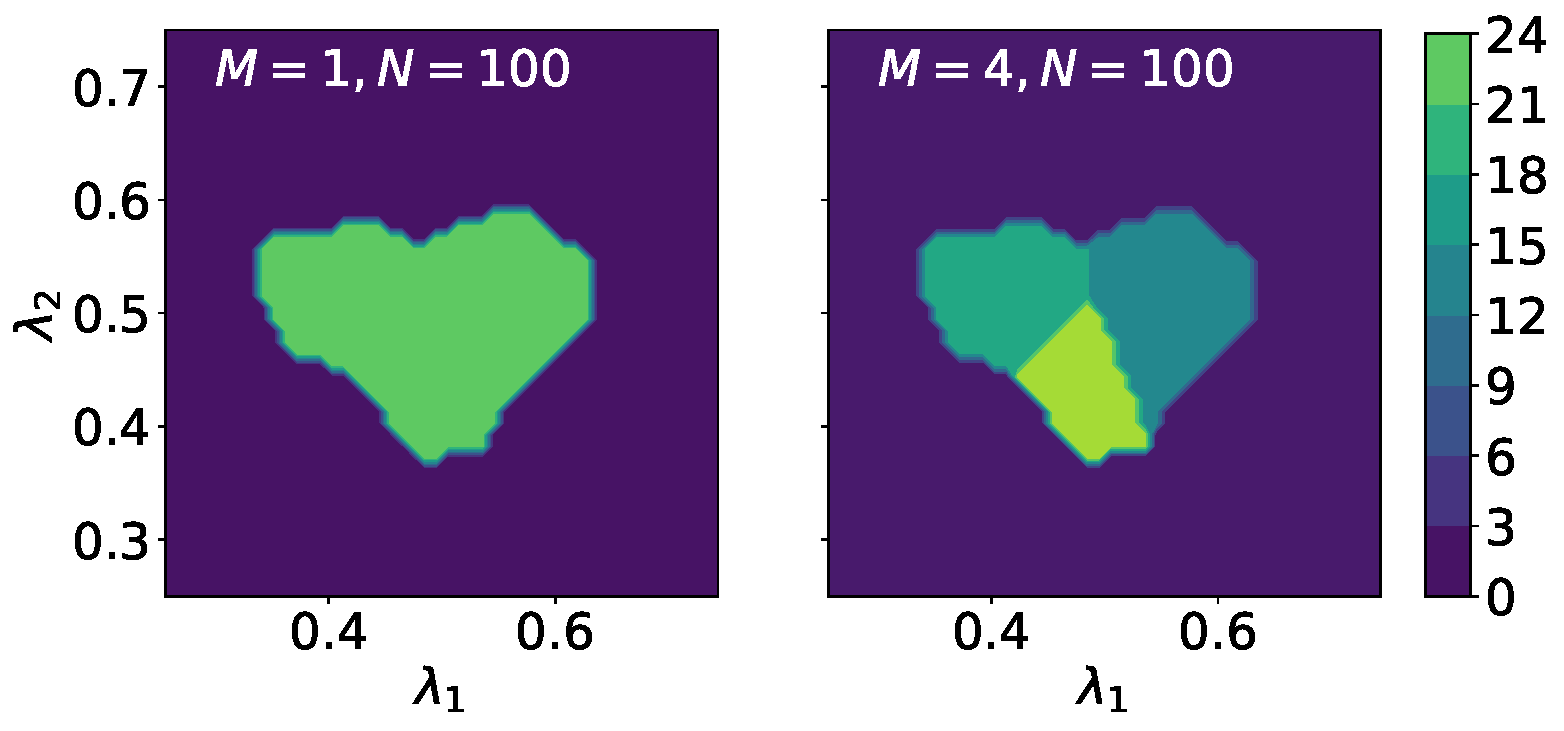
\includegraphics[width=\linewidth]{./examples/identity/set/M1-N100_N100-vs-M4-N100_N100.pdf}
\end{minipage}
\caption{
$\nsamps=100$ were used to discretize $\pspace$ and $\ndiscs=1, 4$ (left/right) were used to discretize $\dspace$.
The latter was chosen to visualize the geometry of describing $\pspace$ with $\pborel$.
}
\label{fig:ex:identity_set_1E2}
\end{figure}

We have chosen a uniform density to describe the uncertainty in our output space.
Any value that is within $0.1$ to the left and right of the reference value \pythoninline{Qref = [0.5, 0.5]} in each dimension is treated as equally likely.
This was done so that using $\ndiscs = 1$ samples to discretize $\dspace$ would fully characterize the characteristic function density representing this uncertainty.
The inverse image of this set is a characteristic function defined on $\pborel$, so errors will exist in particular at the boundaries of the region.

The fundamental challenge with the set-based approach is linked to the geometry of the induced Voronoi-cell tesselation on $\pspace$.
With only $\nsamps = 100$ samples, we see in \ref{fig:ex:identity_set_1E2} that the region (which is supposed to be a square) hardly represents one.
There is ample variation in the shape parameters of the induced sets $\VV_\iparam$ when so few samples are used.
It is possible to ``get lucky'' with the aligning of boundaries between the true target density $\Chi_{[0.4, 0.6]^2}$, but the Figure is representative of the difficulty of using $\nsamps = 100$ random samples to describe a geometry.
With $\nsamps = 1000$, there are usually still significant differences in the symmetric difference of approximated and true supports of the densities.

Below, we demonstrate the use of more samples to resolve the geometry of the desired set.
\begin{figure}[ht]
\begin{minipage}{.975\textwidth}
  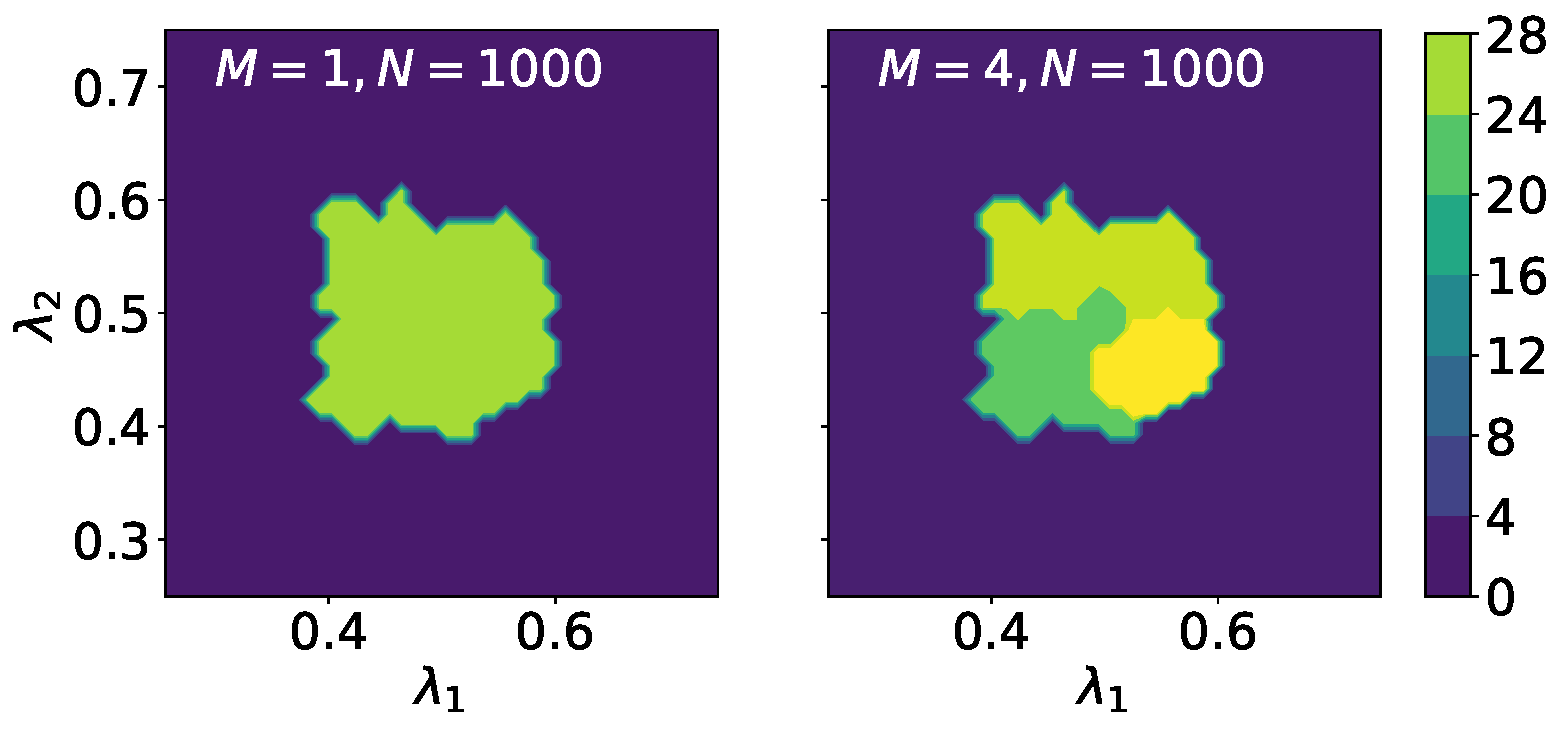
\includegraphics[width=\linewidth]{./examples/identity/set/M1-N1000_N1000-vs-M4-N1000_N1000.pdf}
  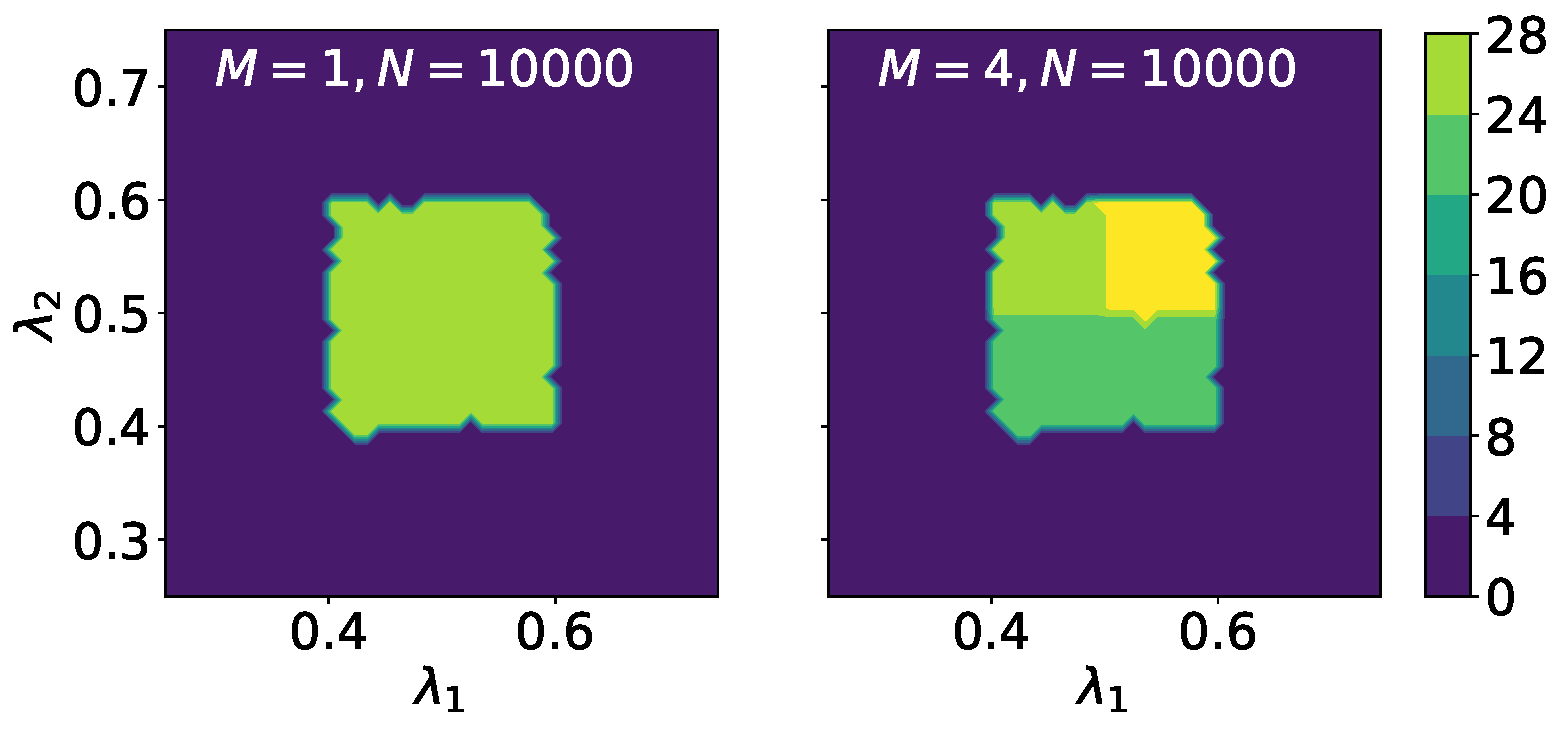
\includegraphics[width=\linewidth]{./examples/identity/set/M1-N10000_N10000-vs-M4-N10000_N10000.pdf}
\end{minipage}
\caption{
(Top):$\nsamps=1,000$ were used to discretize $\pspace$ and $\ndiscs=1, 4$ (left/right) were used to discretize $\dspace$.
(Bottom): The same, except with $\nsamps=10,000$, where we finally begin to see something resembling the correct correct geometry.
}
\label{fig:ex:identity_set_1E3_1E4}
\end{figure}
\FloatBarrier

We remark on the fact that in this particular situation, $\ndiscs = 1$ is a ``correct'' choice for the probability measure chosen, and $\ndiscs = 4$ actually introduces errors.
The reason that the latter solutions have different values inside of the support of $\PPspace$


%%%%%%%%%%%%%%%%%%%%%%%%%%%%%%%%%%%%%%%%%%%%%%%%%%%%%%%%%%%%%%%%%%%%%%
\pagebreak
\section{Sample-Based Inversion for Measures}\label{sec:ch02-sample}
[TK - Words]

\begin{equation}
\updatedP = \initialP \frac{\observedP}{\predictedP}
\end{equation}

\begin{equation}
\begin{split}
\dci\\
\dciP\\
\dciD
\end{split}
\end{equation}

In place of the ansatz, we have an initial distribution.

\subsection{Numerical Approximation and Analysis}\label{sec:sample-approx}


\vspace{2in}

\subsection{Descriptions of Error}\label{sec:sample-error}

KDE is now the primary source, show relevant triangle inequality here.
Summarize Troy and Tim's work on the sensitivity analysis of everything.


Then, we have by repeated application of the triangle inequality that
\begin{equation}
\label{eq:sample-triangleineq}
d(\PP_{\pspace, \ndiscs, \nsamps, h}, \paramP) \leq
\underset{ \text{(E1)} }{\underbrace{d(\PP_{\pspace, \ndiscs, \nsamps, h},\PP_{\pspace, \ndiscs, \nsamps})}} +
\underset{ \text{(E2)} }{\underbrace{d(\PP_{\pspace, \ndiscs, \nsamps}, \PP_{\pspace, \ndiscs}) }}+
\underset{ \text{(E3)} }{\underbrace{d(\PP_{\pspace, \ndiscs}, \paramP) }}.
\end{equation}

Talk more about it.

\vspace{2in}

\subsection{Example}\label{sec:sample-example}
Identity Map in two dimensions


Talk about the problem setup, code blocks shown.

\begin{python}
"""
Set up and solve problem with identity map
"""
# import libraries
import bet.sample as sample
import bet.sampling.basicSampling as bsam
import numpy as np
import scipy.stats as sstats

# define input space parameters and model to instantiate sampler object
dimension = 2
numSamples = 100
I = np.eye(dimension)
def model(input_samples):
        return (I@input_samples.T).T
sampler = bsam.sampler(model)

# instantiate objects that hold input/output samples
input_set = bsam.random_sample_set('r', dimension, num_samples=numSamples)
disc = sampler.compute_QoI_and_create_discretization(input_set)

# define inverse problem
disc.set_initial(dist=sstats.uniform, loc=0, scale=1, gen=False)
disc.set_observed(dist=sstats.uniform, loc=0.4, scale=0.2)

disc_a = disc.copy()
# set analytical density (dimension is inferred)
disc_a.set_predicted(dist=sstats.uniform, loc=0, scale=1)

# create different sample sets with higher fidelity
disc_b = disc.copy()
disc_b.set_initial(num=int(1E3), gen=True)
# the line above removes the previous predicted distribution,
#     stored densities, probabilities, and volumes.
disc_c = disc.copy()
disc_c.set_initial(num=int(1E4), gen=True)
\end{python}

Note that there is no need to explictly call {\tt disc.compute\_pushforward()}, (or \pythoninline{disc.compute_predicted()}) since it is computed automatically if none have been previously constructed.
When \pythoninline{disc.updated_pdf()} is called, densities are evaluated at the initial set of $\nsamps$ random samples, and stored in \pythoninline{disc._input_sample_set._densities}.
However, the function \pythoninline{disc.predicted_pdf()} is capable of evaluating the solution at any new set of samples (provided a model is available/equipped to the discretization), something we leverage for plotting on a regular grid.

Once our four discretization objects \pythoninline{disc}, \pythoninline{disc_a}, \pythoninline{disc_b} and \pythoninline{disc_c} have been generated, we can use some utility plotting functions to compare the densities:

\begin{python}
"""
Plotting code to generate figures.
"""
# define plotting parameters
nbins = 50
xmn, xmx = 0.25, 0.75
ymn, ymx = 0.25, 0.75
xi, yi = np.mgrid[xmn:xmx:nbins*1j, ymn:ymx:nbins*1j]
# plotting functions call .get_updated(), which re-computes
# the pushforward distribution on a regular grid of samples
plot_2d_comparison(xi, yi, disc, disc_a, '$N=$100', 'Analytical')
plot_2d_comparison(xi, yi, disc_b, disc_c, '$N=$1,000', '$N=$10,000')
for d in [disc, disc_b, disc_c]:
    udpated_pdf_conditional_comparison(d, num=100, condition_on=0.5, label='approx')
\end{python}

\begin{figure}[ht]
\begin{minipage}{.975\textwidth}
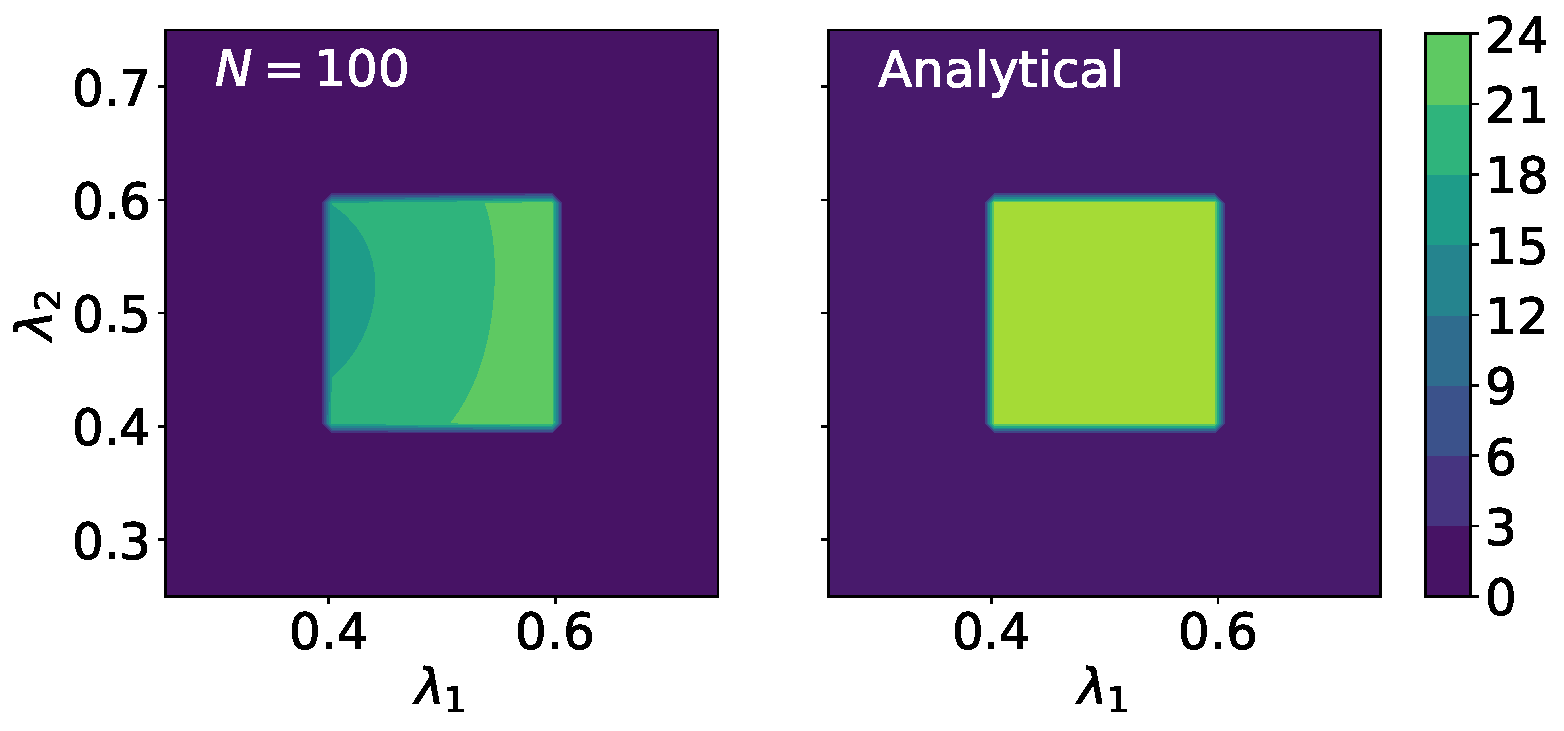
\includegraphics[width=\linewidth]{./examples/identity/samp/N100_N100-vs-Analytical_N100.pdf}
\end{minipage}
\caption{
(Left): $\nsamps=100$ were used to construct the predicted distribution $\predicted$.
(Right): By specifying an analytical $\predicted$, the effect of using $\nsamps$ to approximate a pushforward distribution disappears. The problem can be fully specified in BET without any random sampling.
}
\label{fig:ex:identity_sampling_exact}
\end{figure}

\begin{figure}[ht]
\begin{minipage}{.975\textwidth}
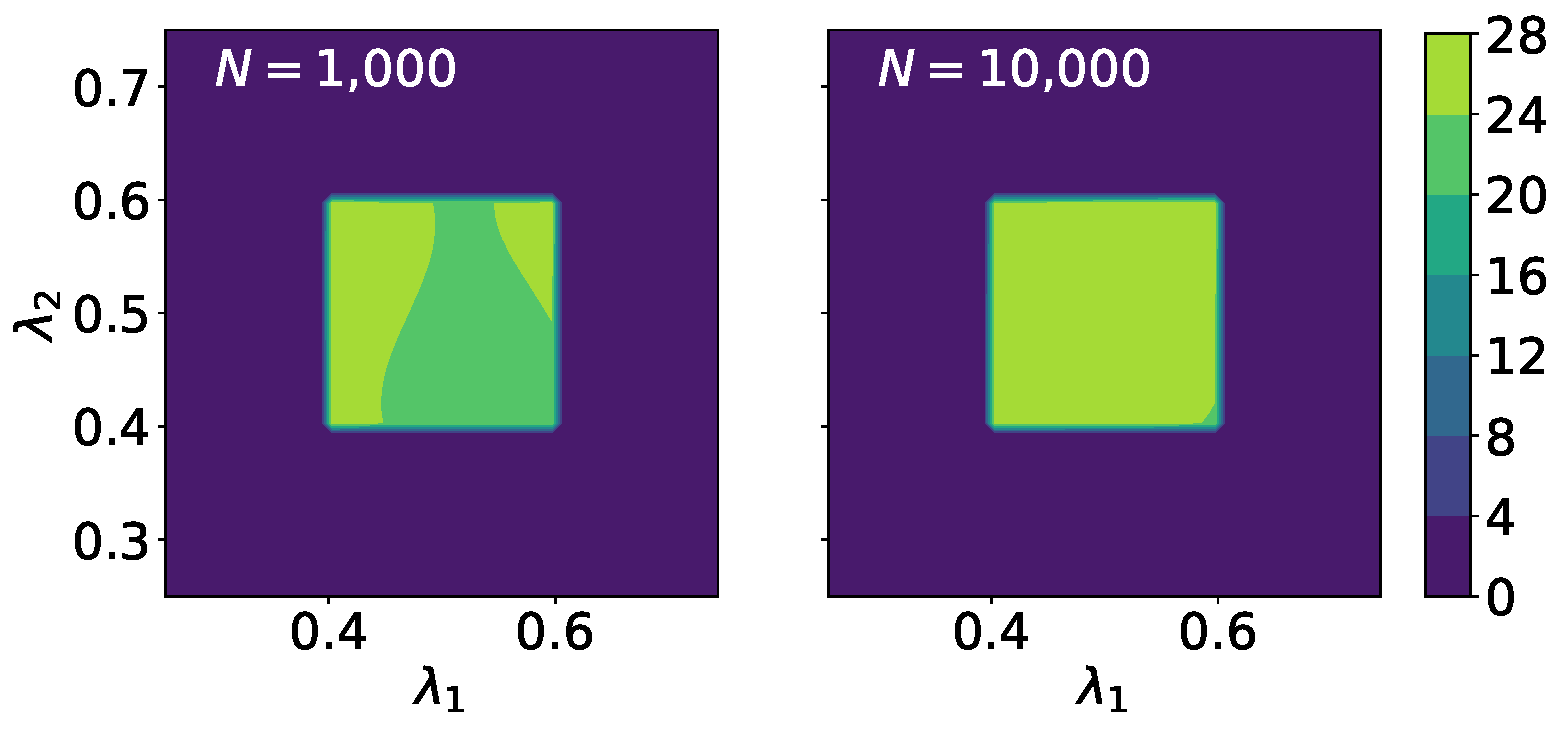
\includegraphics[width=\linewidth]{./examples/identity/samp/N1-000_N1000-vs-N10-000_N10000.pdf}
\end{minipage}
\caption{
$\nsamps=1,000$ (left) and $\nsamps=10,000$(right) were used to construct the predicted distribution $\predicted$.
There is no signficant error in estimating the support of the distribution, only the density approximation itself.
}
\label{fig:ex:identity_sampling_approx}
\end{figure}

\begin{figure}[ht]
\centering
	\begin{minipage}{.315\textwidth}
		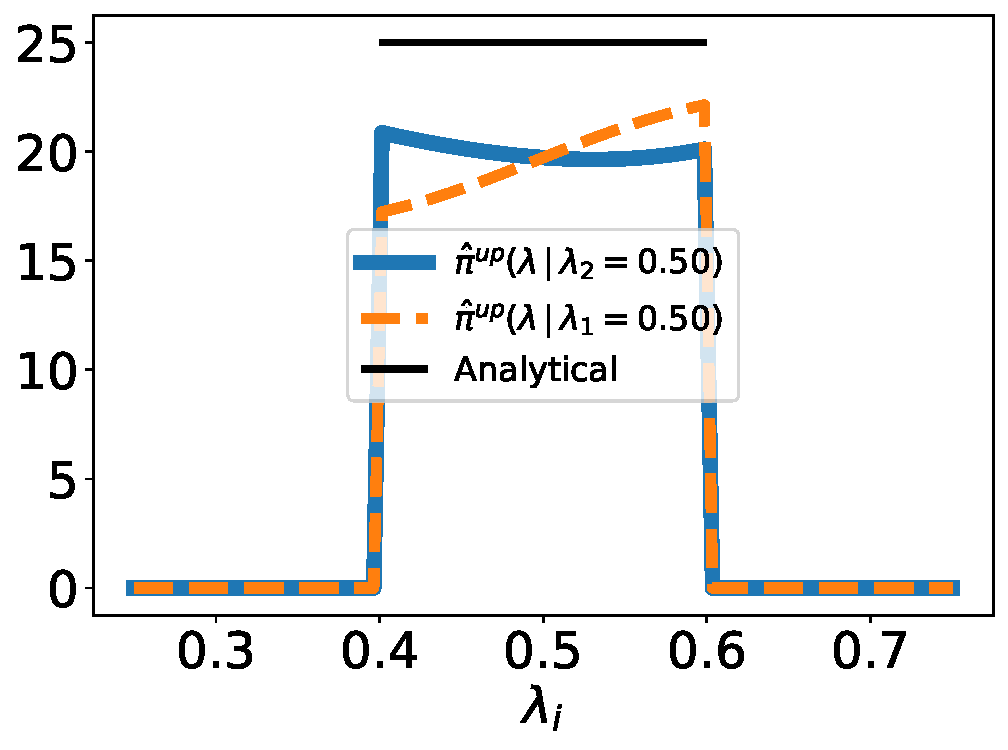
\includegraphics[width=\linewidth]{./examples/identity/samp/identity_1d_conditionals_50E-2_N100_approx.pdf}
	\end{minipage}
	\begin{minipage}{.315\textwidth}
		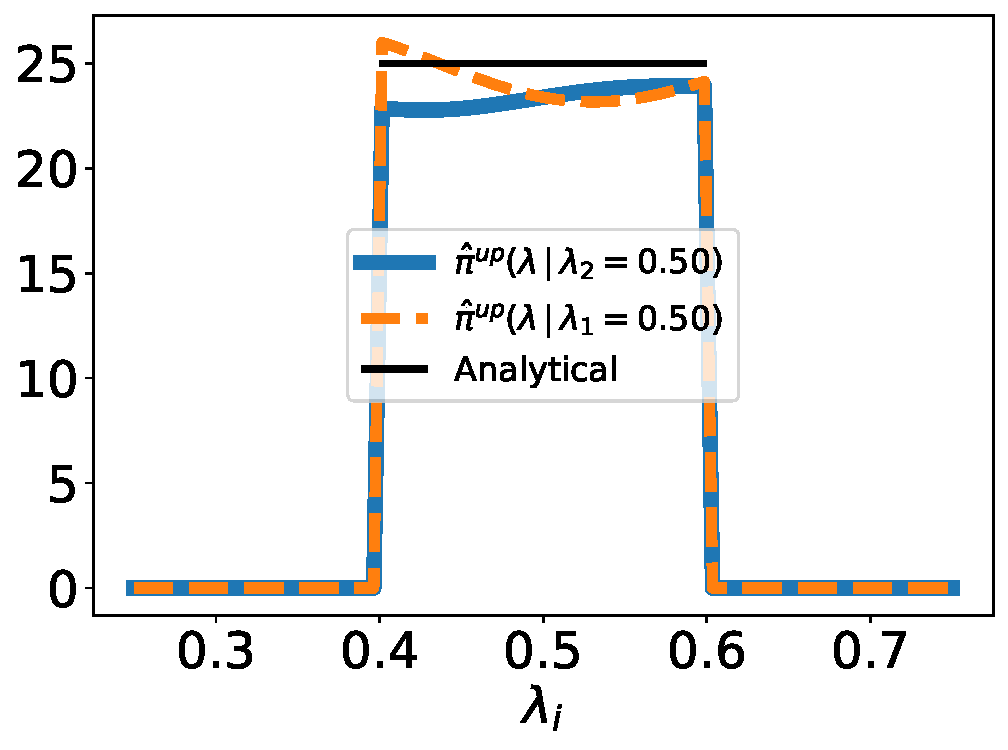
\includegraphics[width=\linewidth]{./examples/identity/samp/identity_1d_conditionals_50E-2_N1000_approx.pdf}
	\end{minipage}
  \begin{minipage}{.315\textwidth}
		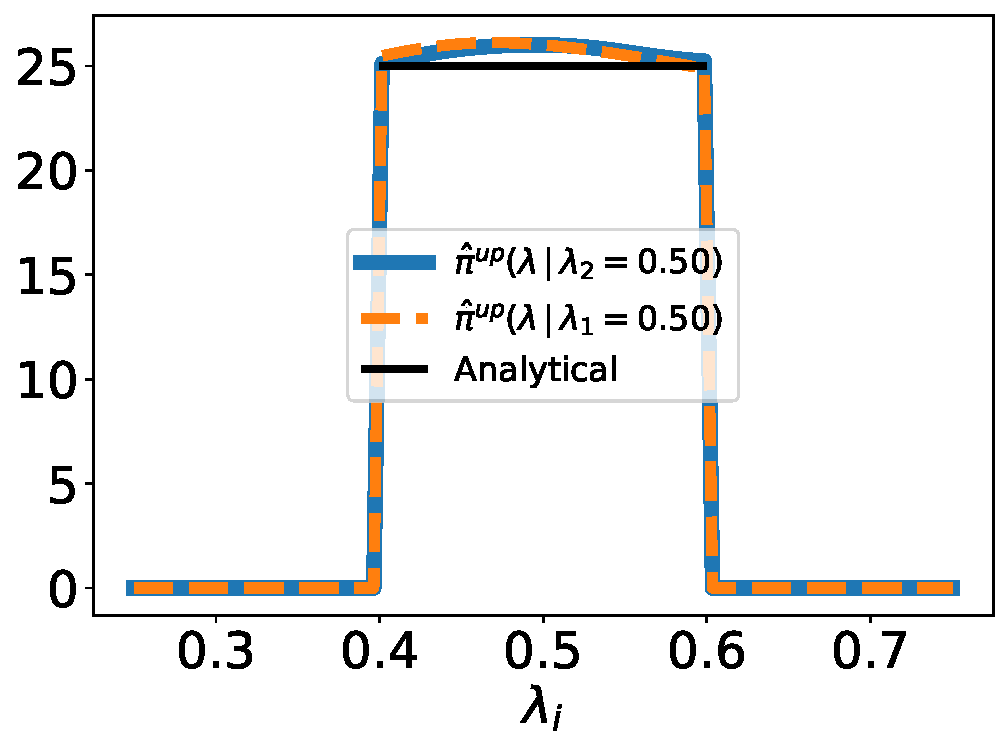
\includegraphics[width=\linewidth]{./examples/identity/samp/identity_1d_conditionals_50E-2_N10000_approx.pdf}
	\end{minipage}
\caption{
(Left to right, respectively): Conditionals passing through $(0.5, 0.5)$ for $\predicted$'s generated with $\nsamps=1E2, 1E3, \text{ and } 1E4$ random samples.
}
\label{fig:identity_sampling_conditionals}
\end{figure}
\FloatBarrier


%%%%%%%%%%%%%%%%%%%%%%%%%%%%%%%%%%%%%%%%%%%%%%%%%%%%%%%%%%%%%%%%%%%%%%

\
\section{Software Contributions}\label{sec:ch02-software}

\subsection{Background and Motivation}
The open-source software package BET was developed actively from 2012-2015 as part of research performed under grant [TK grant-DOE].
It was originally written in Python 2.7 and is administered by the Computational Hydrology Group at the University of Texas: Austin through their UT-CHG GitHub group [TK - cite Github].
The purpose of this open-source software package was to implement the methods first described in [TK - cite BET papers] for the description and solution of stochastic inverse problems.

In the intermittent years since its original publication in [TK - date of first release, cite Github], the BET package has seen two major releases and the incorporation of several sub-modules (e.g. the functions in {\tt sensitivity} implement much of the original research performed by Dr. Walsh [TK - cite Scott]).


\subsection{Upgrades, Updates, and Features}
Since the last major release [TK - cite latest release], the Python community announced the end of long-term support for Python 2 [TK - cite announcement].
Several of the dependencies in BET have been actively developed in Python 3 with no updates to the Python 2 analogs, which suggested that BET should likely undergo the same transition.

The work summarized in Section~\ref{sec:ch02-sample} was implemented in Python 3 independently by the author through the release of the ConsistentBayes package.
Since that code was used for many of the results that constituted the preliminary results for this work, it made very litle sense to re-implement them in Python 2 for BET given the recent trends in community development.
With funding made available through NSF [TK - cite grant], the opportunity to upgrade BET to Python 3 was the most sensible choice.


\subsubsection{Version 2.1.0}
The upgrade to Python 3.4+ began in January 2019 as a first step to incorporate the new sample-based method into BET.
It was completed in late February.
Major (minor? version? TK) release 2.1.0 [TK - put in release] was designed to provide backwards-compatibility with the Python 2.7 version.
Future installations (starting in 2020) will not limit the versions of some core dependencies in order to accomodate backwards-compatibility with Python 2 (e.g. {\tt numpy}, {\tt scipy}), since this would likely downgrade previously installed software for end-users.


\subsubsection{Version 2.2.0}
Several releases of BET (after the upgrade to Python 3 in v2.1.0), incorporated developments that will be discussed herein.
For


\subsubsection{Version 2.2.1}
Major bugfix for parallel testing allowed tests to pass for more than 2 processors.
For some tests, this involved changing the setup parameters to ensure the problem was large enough to break up onto up to 8 processors.
For others, siginficant changes had to be made to structure to allow for proper saving and loading of files in parallel.


\subsubsection{Version 2.3.0}
This release incorporated the sampling-based approach first dicussed in Section~\ref{sec:ch02-sec:ch02-sample}.


\subsection{Examples in BET}
Basic plotting functionality of BET is demonstrated in iPython notebooks [TK - some kind of citation here], which have seen an exponential growth rate on GitHub, and can be edited by the end-user to work with different plotting library versions and backends.
These notebooks were originally created to reflect the example suite in BET (which were {\tt .py} files), but later they were migrated into a separate repository BET-examples to allow for better organization.
In the new framework, each notebook functions as an independent example.
Several of these notebooks were adapted from the example code in this thesis repository.


\section{Illustrative Examples}\label{sec:ch02-examples}
In some examples, we do not work with any model $\M$ and make observations $\qoi$ directly on the data space $\dspace$, so term (E1) in Eq.~\eqref{eq:set-triangleineq} is identically zero for the examples we present in Section \ref{sec:ch02-examples}.
Furthermore, since the probabilities we introduce on $\dspace$ in the numerical results are uniform and our maps linear, the densities can be described analytically with a characteristic function.
In this event, the solution $\paramP$ to the SIP can be given exactly by a change of variables formula, so the inverse set can be known exactly.
When we invert characteristic functions, our solutions will also be members of this same family if the choice of \emph{ansatz} (or \emph{initial density}) is taken to be uniform over $\pspace$.
These examples allow us to study the DCI method for a class of functions for which a solution is readily available, and serves as a requisite testing ground before advancing to more nuanced problem definitions.
We present a brief overview of the factors that influence our practical ability to accurately approximate $\paramP$ and $\updated$ using finite sampling.

For the set-based approach discussed in \ref{sec:ch02-set}, it is desirable that $\ndiscs$ is chosen without respect to $\nsamps$ so that (E3) = $d(\PP_{\pspace, \ndiscs}, \paramP)$ from \ref{sec:set-error} has been made sufficiently small or eliminated entirely.
This amounts to saying that the decision about how to discretize the uncertainty in $\dspace$ is made a priori to cater to some problem specifications.
We choose to impose uniform distributions on $\dspace$ so that the set-valued analog to $\observed$ is perfectly described with $\ndiscs=1$.
Therefore, we focus our attention on the source of error introduced by $d(\PP_{\pspace, \ndiscs, \nsamps}, \PP_{\pspace, \ndiscs} )$, the primary contribution of error in Eq.~\eqref{eq:set-triangleineq}, which is given by the term (E2) = $d(\PP_{\pspace, \ndiscs, \nsamps}, \PP_{\pspace, \ndiscs})$.

Since there is no error introduced from discretizing $\pspace$ in the sample-based approach from \ref{sec:ch02-sample}, the term (E2) is not what contributes to error in the sample-based approach.
As discussed in \ref{sec:sample-error}, the impact of $\nsamps$ is on our ability to characterize $\dspace$.
In situations where an analytical $\predicted$ is not known, we must rely on some form of density estimation.


\subsection{Exponential Decay}\label{ex:decay-set-sample}

To demonstrate the qualitative differences in the solutions provided by the set-- and sample--based methods for a nonlinear problem, we consider an exponential decay problem with uncertain decay rate and initial condition (which are paired to form the 2-D vector $\param$):
$$
\begin{cases}
  \frac{\partial u}{\partial t} & = \param_1 u(t), \\
  u(0) &= \param_2.
\end{cases}
$$

The solution is described by
\begin{equation}
  u(t;\param) = u_0\exp(\param_1 t), \; u_0 = \param_2 ,
\end{equation}

and a nominal value of $\param = 0.5$ is used to simulate the system.
We take a single observation at $t=0.5$s and assume a uniform density with interval length $0.2$ centered at $u(1,0.5)$ to represent the uncertainty in the measurement equipment.
We assume a uniform ansatz / initial density over the unit domain.
We use $N=50$ parameter samples to establish a coarse solution in Figure~\ref{fig:heatrod-sol-ex1}.


\begin{figure}
\begin{minipage}{.475\textwidth}
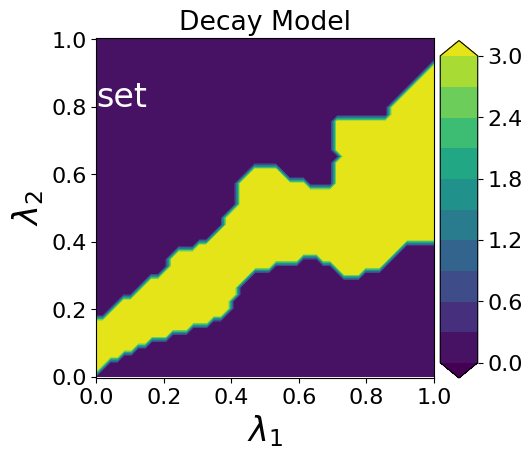
\includegraphics[width=\linewidth]{examples/fig_decay_q1/DecayModel--set_N50_em.png}
\end{minipage}
\begin{minipage}{.475\textwidth}
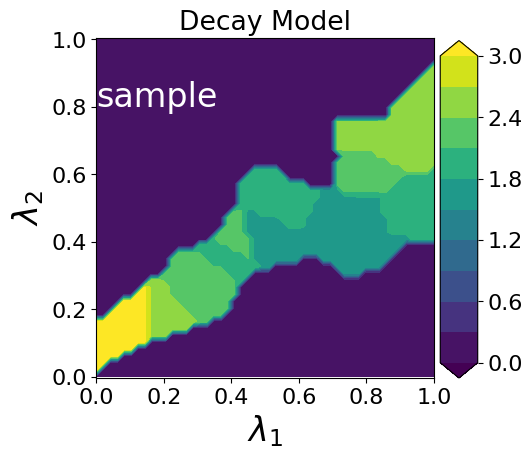
\includegraphics[width=\linewidth]{examples/fig_decay_q1/DecayModel--sample_N50_mc.png}
\end{minipage}
\caption{Observation taken at $t=1$s. The inverse image of the reference measure for set-based (left) and sample-based (right) solutions for $\nsamps=50$ parameter samples.}
\label{fig:heatrod-sol-ex1}
\end{figure}

The decay rate $\param_1$ shows little reduction in uncertainty overall.
If one were to look at marginals of the components of $\param$, it would not appear as if much was learned.
However, the relationship \emph{between} these two quantities has very certainly been elucidated by the solution of the inverse problem.
Where once $\pspace$ was a rectangular region, the set of possible parameters has been reduced to a diagonal band.
The sample-based approach, especially at this low sample size (density estimation in 2-D at $50$ samples is a stretch), has some visible downsides.
It does not capture the equivalence--class nature of the solution set the way the set--valued one does, which benefits from using $\ndiscs=1$ (aligning with the choice of uniform observed density).


We address what would occur had we been able to observe earlier in time at $t=0.5$ by showing the associated solutions under the same experimental conditions in \ref{fig:heatrod-sol-ex2}.
There is a marked reduction in uncertainty, as several regions of $\pspace$ have been ruled out from consideration.


\begin{figure}
\begin{minipage}{.475\textwidth}
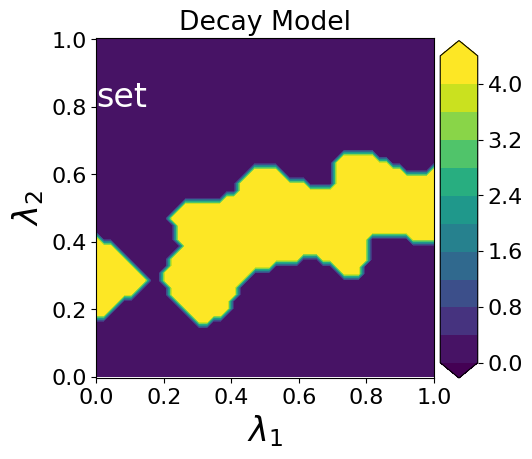
\includegraphics[width=\linewidth]{examples/fig_decay_q2/DecayModel--set_N50_em.png}
\end{minipage}
\begin{minipage}{.475\textwidth}
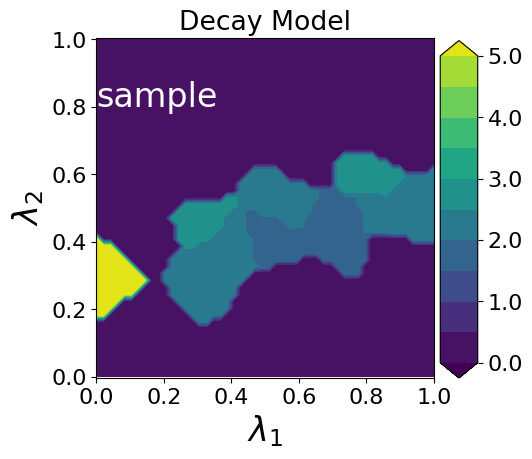
\includegraphics[width=\linewidth]{examples/fig_decay_q2/DecayModel--sample_N50_mc.png}
\end{minipage}
\caption{Observation taken at $t=0.5$s. The inverse image of the reference measure for set-based (left) and sample-based (right) solutions for $\nsamps=50$ parameter samples.}
\label{fig:heatrod-sol-ex2}
\end{figure}


Observing earlier in time helps especially in reducing the (marginal) values for the initial condition $\param_2$, while the rate $\param_1$ is still to some degree able to take any values in its original domain.
Both solution types suffer from discretization error, as evidenced by the break in the contour structure.
By comparison to \ref{fig:heatrod-sol-ex1}, there is more more confidence in the solution (represented by the reduced support of the image).

However, at $\nsamps=50$, the sample--based approach struggles to assign uniform probability to different contour events.
This may suggest that in situations with very limited model evaluation budget and set-valued solutions involving uniform uncertainties in measurements, the set-valued approach may serve a useful purpose.


\subsection{1D Heat Rod}\label{ex:heat-set-sample}

Consider the one-dimensional heat equation with homogeneous Neumann boundary conditions on the unit interval:

\begin{equation}
\begin{split}
\rho c \frac{\partial T}{\partial t} = \nabla \cdot ( \kappa \nabla T) + f(x), \quad & x\in (0,1), t\in (0,1) \\
f(x) = A e^\frac{- (x-0.5)^2}{w} \Chi_{[0,0.5]}(t)
\end{split}
\end{equation}
\emph{Alternative setup: }

\begin{equation}
\begin{cases}
\rho c \frac{\partial T}{\partial t} = \nabla \cdot ( \kappa \nabla T) + f(x,t), & \text{if } x\in \Omega \\
\frac{\partial T}{\partial \vec{n}} = 0 & \text{if } x\in \partial \Omega
\end{cases}
\end{equation}
where $\Omega = (0,1)\times (0,1)$ is the space-time interior and $f(x,t) = A e^\frac{- (x-0.5)^2}{w} \Chi_{[0,0.5]}(t)$.

Here, we interpret the following problem as heating the middle of an infinitesimally thin unit-length rod for half a second with the heat-source modeled by a Gaussian curve with amplitude $A=50$ and variance of $w=0.05$.
The rod is subdivided in two, and each half has an uncertain thermal diffusivity $\kappa \in [0.01, 0.2]$.
This yields a two-dimensional parameter space $\param = (\param_1, \param_2) \in [0.01, 0.2]\times [0.01, 0.2]$, where $\param_1$ represents the thermal diffusion on the left-half and $\param_2$ is the $\kappa$ for the right half.

\begin{figure}[h]
\begin{minipage}{.475\textwidth}
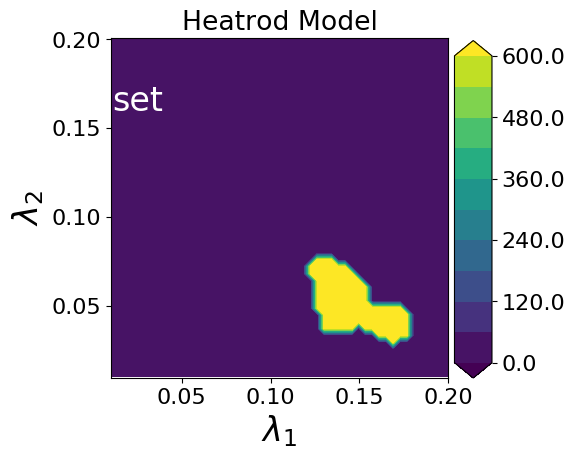
\includegraphics[width=\linewidth]{examples/fig_heatrod_q1/HeatrodModel--set_N50_em.png}
\end{minipage}
\begin{minipage}{.475\textwidth}
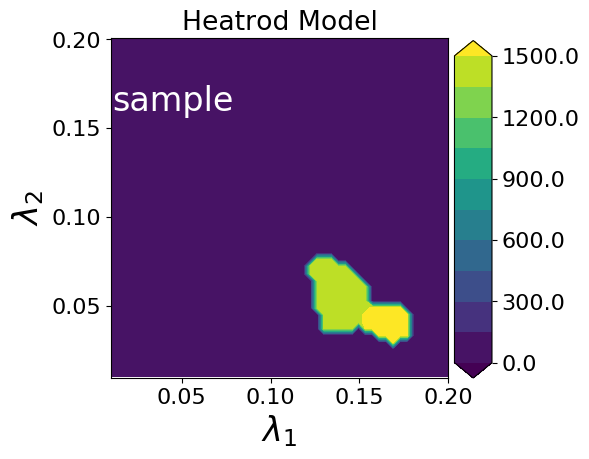
\includegraphics[width=\linewidth]{examples/fig_heatrod_q1/HeatrodModel--sample_N50_mc.png}
\end{minipage}
\caption{The inverse image of the reference measure for set-based (left) and sample-based (right) solutions for $N=50$ parameter samples.}
\label{fig:heatrod-sol-ex}
\end{figure}

